\chapter{\#42 Public Transport in the UK}

\section{Task Explanation}
The objective is to create a network for UK public transport systems, focusing on different types of transport available as CSV datasets. The goal is to generate individual networks for each city, excluding less populated ones. For each city and each layer, two files have been produced: one for nodes (nodeID, latitude, longitude, geometry data) and one for edges (nodeID\_from, nodeID\_to). The challenge lies in integrating two datasets that do not directly correspond with each other.

\section{Methodology}
\textbf{Population Data Redistribution} \\
Due to difficulties in matching nodes to cities using provided datasets, I used counties and travel-to-work areas (TTWAs) instead. The population data were initially at the county level. For a more accurate representation of transport networks, I redistributed the population data using the `st\_intersection` function from the `sf` library, assigning the population to each TTWA proportionally based on the intersection area with the counties. Population data for counties was sourced from the ONS \cite{county_population_data}.
Mathematically, if $A_{i,j}$ is the area of intersection between county $i$ and TTWA $j$, and $P_i$ is the population of county $i$, the population assigned to TTWA $j$ from county $i$ is:
\begin{equation}
 P_{i,j} = P_i \times \frac{A_{i,j}}{A_i}
\end{equation}
where $A_i$ is the total area of county $i$. The total population for TTWA $j$ is then:
\begin{equation}
 P_j = \sum_i P_{i,j}
\end{equation}

\noindent \textbf{Precision and Recall Test} \\
To verify the accuracy of this redistribution, I conducted precision and recall tests by comparing the population in TTWAs with the population data for each city sourced from the World Population Review \cite{city_population_data}. Precision is calculated as:
\begin{equation}
\text{Precision} = \frac{TP}{TP + FP}
\end{equation}
Recall is calculated as:
\begin{equation}
\text{Recall} = \frac{TP}{TP + FN}
\end{equation}
The results showed precision of 96.5\% and recall of 97.2\%, indicating the method successfully preserved the total population.

\noindent \textbf{Filtering TTWAs by Population} \\
To focus on significant areas, I excluded TTWAs in the lowest quartile of the population distribution. This threshold is adjustable based on analysis requirements.
\begin{figure}[H]
	\centering
	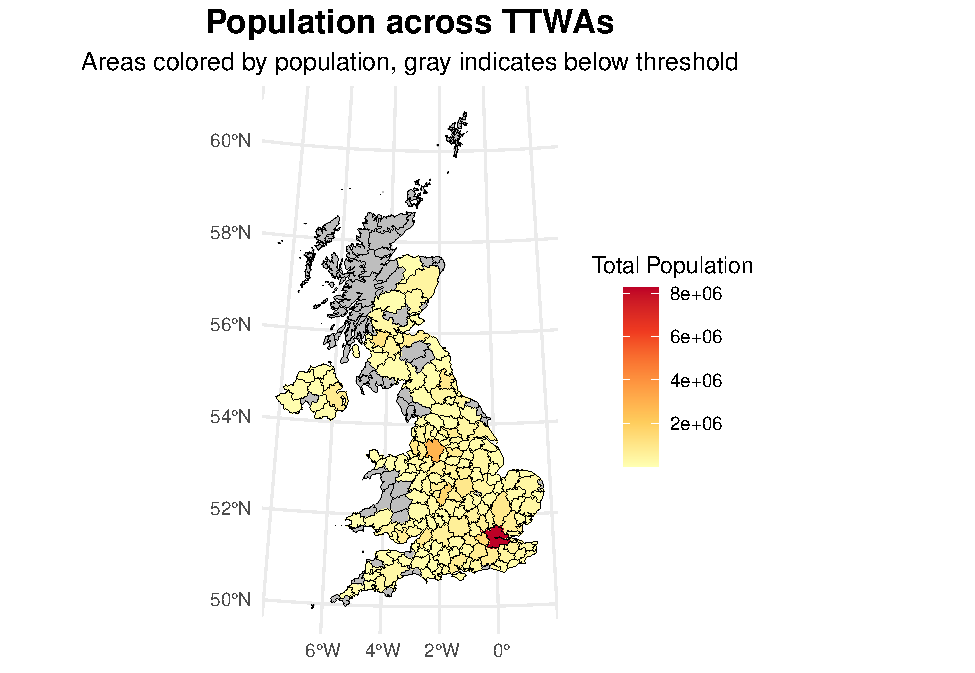
\includegraphics[width=0.8\textwidth]{images/LowedPopulationTTWAs.pdf}
\end{figure}

\noindent \textbf{Creation of Node and Edge Files} \\
I created node and edge files for each TTWA. Nodes were assigned to TTWAs using their geographical coordinates with the `st\_within` function from the `sf` library. Each node file includes nodeID, latitude, longitude, layer, degree, and geometry data for plotting. Edges were attributed to TTWAs based on the nodes they connect. Each edge file includes nodeID\_from, nodeID\_to. This resulted in node and edge files for each TTWA and the entire UK network, enabling detailed analysis at both local and national levels. TTWA boundary data was obtained from the ONS \cite{ttwa_boundary_data}.

\vspace{-1cm}
\begin{figure}[H]
	\centering
	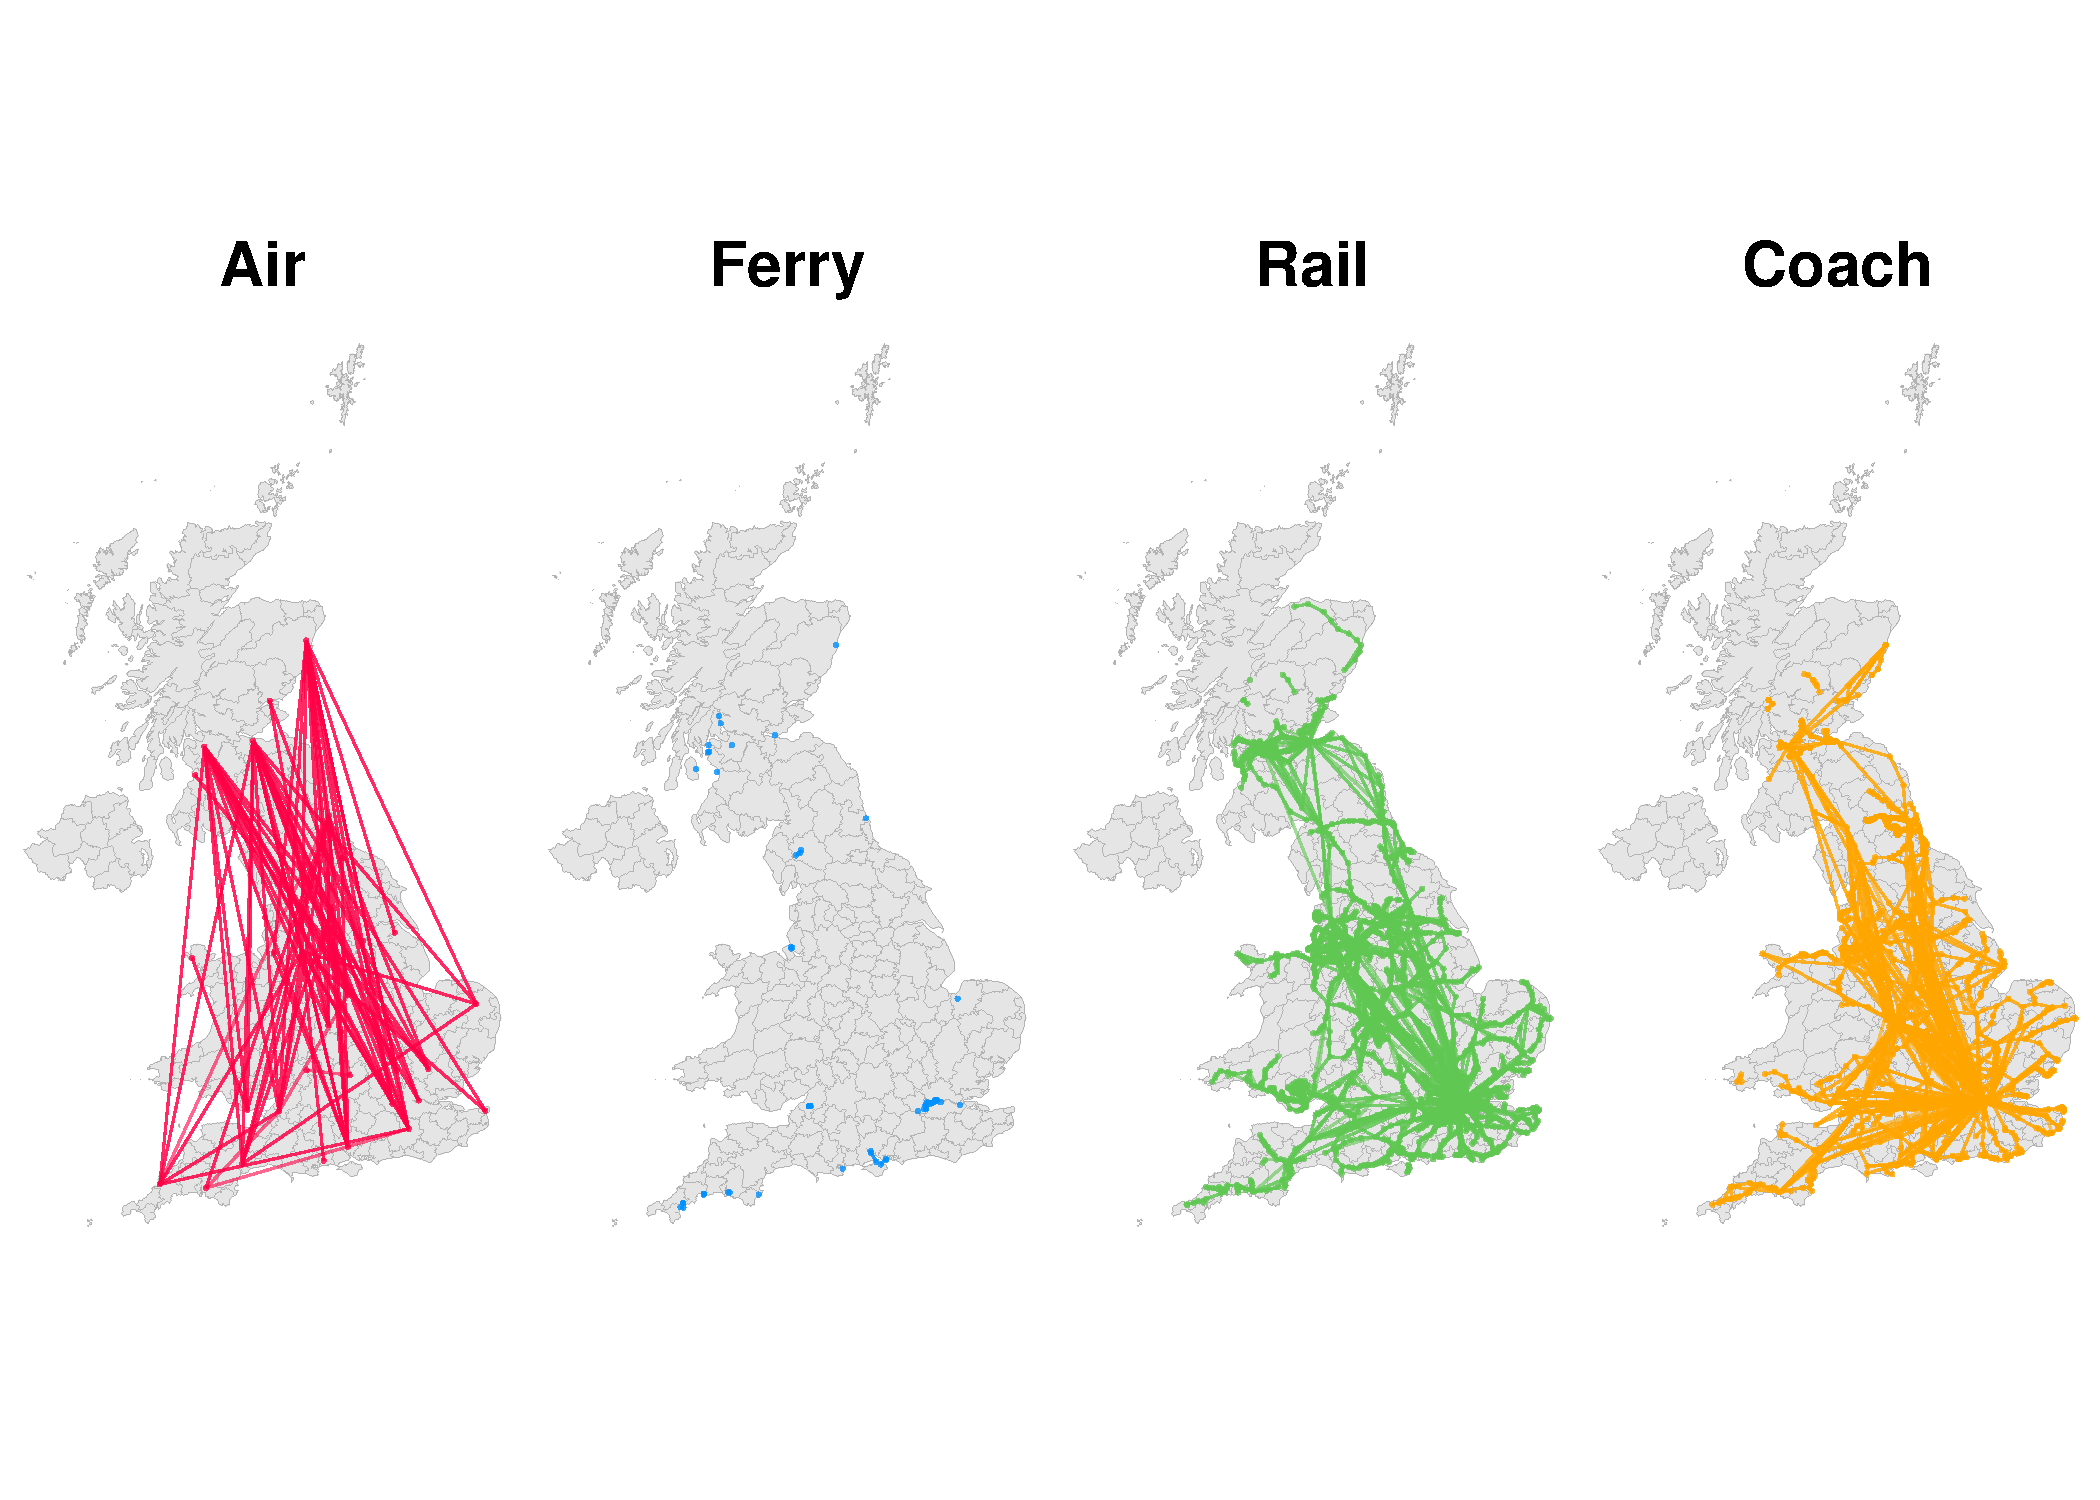
\includegraphics[width=0.8\textwidth]{images/multilayer_network_uk.pdf}
	\caption{Visualization of the UK transport network across multiple layers, highlighting only the most populated regions.}
\end{figure}

\begin{figure}[H]
	\centering
	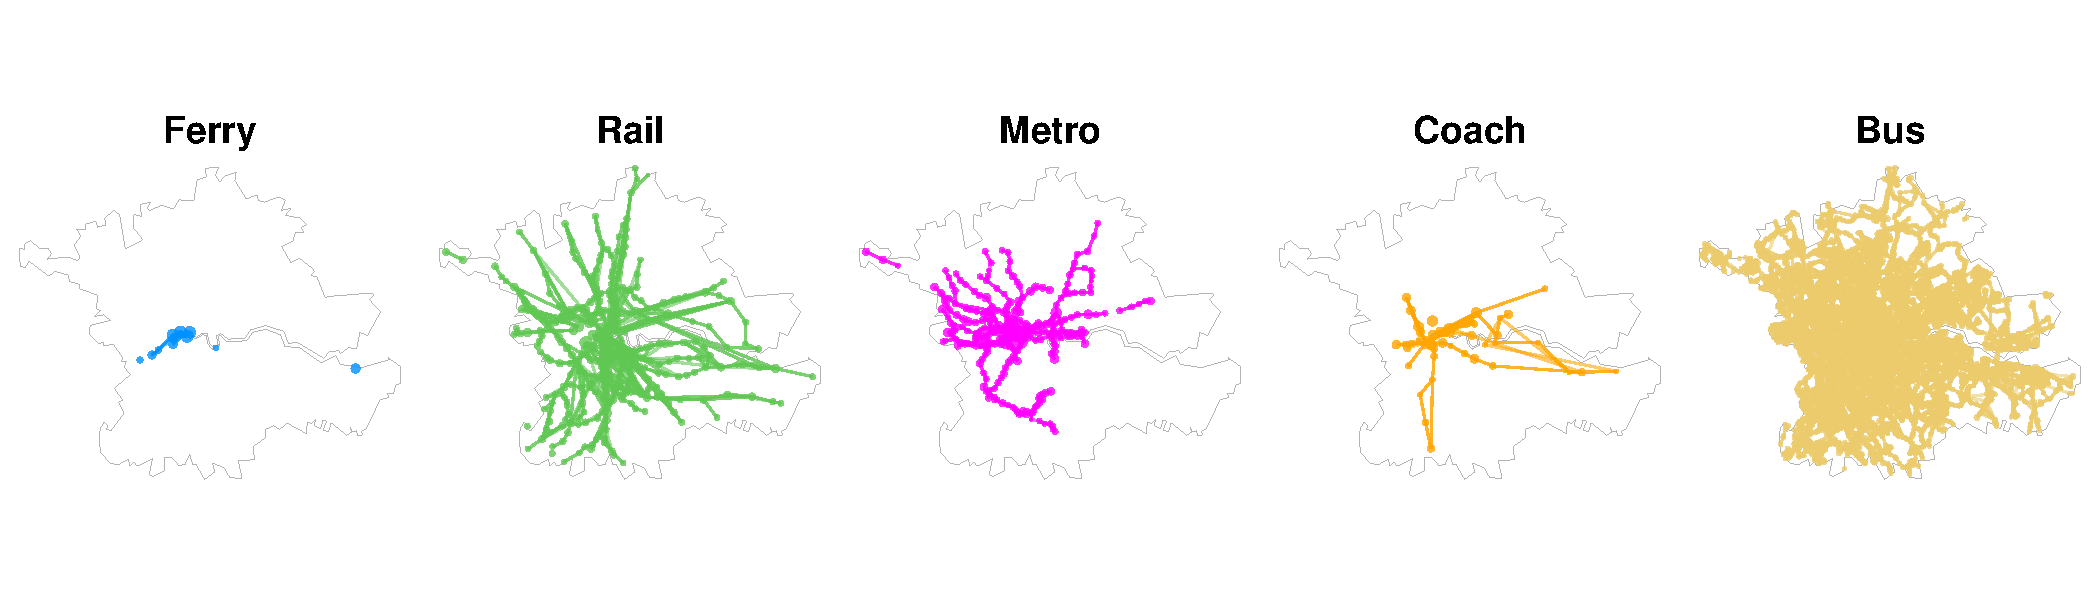
\includegraphics[width=1\textwidth]{images/combined_network_London.pdf}
	\caption{Visualization of London transport network across multiple layers.}
\end{figure}




